\ofsection{Omega Fantasy rules}
%
The following is a collection of optional rules and content for \textbf{Omega~Fantasy}, which you can use to create a closer feeling to Final Fantasy Tactics.
%
\\\\
%
\ofaccent{Grid-based Combat:}
You can use a square grid to visualize combat in the same manner as FFT.
Each square is 1u by 1u in size and player characters take up 1 square of space.
The distance between two squares is the sum of the horizontal and vertical squares between them, this system is called the \textbf{Manhattan~distance}.
In other words, adjacent squares to your up, down left and right have a distance of 1u from you, but adjacent diagonal ones have a distance of 2u.
Ranges and target distances for abilities are adjusted accordingly.
The example below shows the normal (2u) target shape, as well as the special shapes line (5u) and front (2u). 
The blue squares represent the caster, while the red ones represent enemy combatants.
%
\vspace*{-0.65cm}\\
%
\begin{figure}[h!]
	\centering
	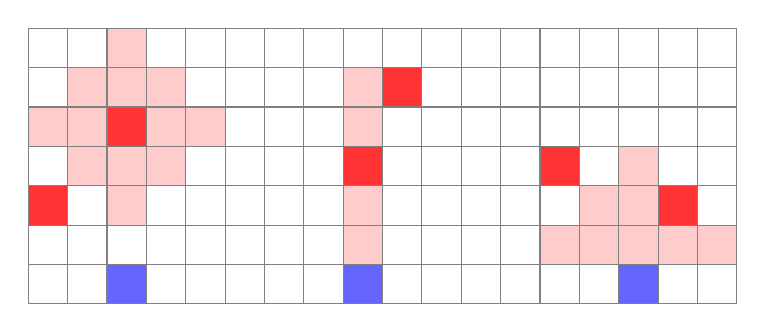
\begin{tikzpicture}[]
	\tikzstyle{filled}=[draw, black!50!white, rectangle, thin, minimum height = 0.5cm, minimum width=0.5cm]
	\tikzstyle{target}=[fill=red!20!white]
	\tikzstyle{caster}=[fill=blue!60!white]
	\tikzstyle{enemy}=[fill=red!80!white]	
	\draw[step=0.5,black!50!white, thin,xshift=-0.25cm,yshift=-0.25cm] (0,0) grid (9, 3.5);	
	%Normal
	\node[filled, caster](g0)at (1, 0) {};
	\node[filled, enemy](g0)at (1, 2) {};
	\node[filled, enemy](g0)at (0, 1) {};
	\node[filled, target](g0)at (1, 1) {};
	\node[filled, target](g0)at (1, 1.5) {};
	\node[filled, target](g0)at (1, 2.5) {};
	\node[filled, target](g0)at (1, 3) {};
	\node[filled, target](g0)at (1.5, 2.5) {};
	\node[filled, target](g0)at (0.5, 2.5) {};
	\node[filled, target](g0)at (1.5, 1.5) {};
	\node[filled, target](g0)at (0.5, 1.5) {};
	\node[filled, target](g0)at (1.5, 2) {};
	\node[filled, target](g0)at (2, 2) {};
	\node[filled, target](g0)at (0, 2) {};
	\node[filled, target](g0)at (0.5, 2) {};
	%Line
	\node[filled, caster](g0)at (4, 0) {};
	\node[filled, enemy](g0)at (4, 1.5) {};
	\node[filled, enemy](g0)at (4.5, 2.5) {};
	\node[filled, target](g0)at (4, 0.5) {};
	\node[filled, target](g0)at (4, 1) {};
	\node[filled, target](g0)at (4, 2) {};
	\node[filled, target](g0)at (4, 2.5) {};	
	%Front
	\node[filled, caster](g0)at (7.5, 0) {};
	\node[filled, enemy](g0)at (8, 1) {};
	\node[filled, enemy](g0)at (6.5, 1.5) {};	
	\node[filled, target](g0)at (7.5, 0.5) {};
	\node[filled, target](g0)at (7.5, 1) {};
	\node[filled, target](g0)at (7.5, 1.5) {};
	\node[filled, target](g0)at (8, 0.5) {};
	\node[filled, target](g0)at (8.5, 0.5) {};
	\node[filled, target](g0)at (7, 0.5) {};
	\node[filled, target](g0)at (6.5, 0.5) {};
	\node[filled, target](g0)at (7, 1) {};
	\end{tikzpicture}
\end{figure}
%
\vspace*{-0.3cm}\\
%
\ofaccent{Directional Defense:}
In conjunction with a square grid, you can also change the potency of a combatant's defense depending on the direction they are attacked from.
At the end of every turn, combatants have to announce the direction that they are facing. 
There are 4 possible directions (up, down, left and right), so the one they are facing is their front, the opposite direction is their back and the two remaining directions are their sides. 
Whenever combatants are Attacked from a side, their DEF is halved when calculating the suffered damage.
Whenever combatants are Attacked from behind, their Evasion DC is increased by 2 while trying to evade the Attack.
%
\\\\
%
\ofaccent{Monsters of Ivalice:}
Below are examples of monsters that are common in the world of Ivalice.
Apart from these, the following monsters from the Omega Fantasy core book may also be encountered:
Chocobo, Skeleton, Ghoul, Cockatrice, Ahriman, Bomb, Coeurl, Mindflayer, Malboro, Behemoth, Red Dragon.
%
\ofrow
%
\ofmonster{Floating Eye}{4}{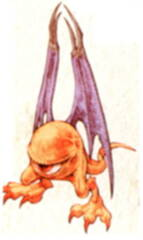
\includegraphics[width=0.16\textwidth]{./art/monsters/eye.jpg}}
{
	HP: & \hfill 32 & MP: & \hfill 30 \\
	STR: & \hfill 2 & DEF: & \hfill 2 \\
	MAG: & \hfill 5 & RES: & \hfill 4 \\
	AGI: & \hfill 4 & Size: & \hfill S\\
}
{\textbf{Beam}: 2d DMG, 3u Range \hfill \textbf{Drops:} 350 Gil}
{	
	\mtech{Wing Buffet}{5}{0r}{3u (front)}{Self}{Enemies in the target area suffer 2d wind damage.}{}
}
%
\pagebreak\\
%
\ofmonster{Goblin}{2}{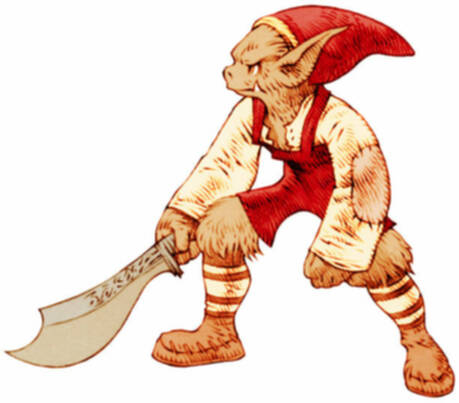
\includegraphics[width=0.26\textwidth]{./art/monsters/goblin.jpg}}
{
	HP: & \hfill 16 & MP: & \hfill 12\\
	STR: & \hfill 2 & DEF: & \hfill 1 \\
	MAG: & \hfill 0 & RES: & \hfill 0 \\
	AGI: & \hfill 3 & Size: & \hfill M\\
}
{\textbf{Knife}: 1d DMG \hfill \textbf{Drops:} 200 Gil}
{
	\mtech{Goblin Punch}{2}{0r}{Single}{Weapon}{Make an Attack against the target. If you hit, you push him back by 1u on top of the damage dealt.}{}		
	\mtech{Spin Punch}{4}{0r}{1u}{Self}{Make an Attack against everyone within 1u.}{}		
}
%
\ofmonster{Red Chocobo}{3}{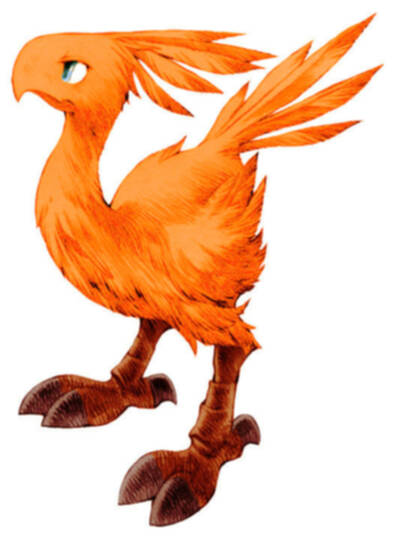
\includegraphics[width=0.18\textwidth]{./art/monsters/chocobo-red.jpg}}
{
	HP: & \hfill 28 & MP: & \hfill 16\\
	STR: & \hfill 3 & DEF: & \hfill 2 \\
	MAG: & \hfill 1 & RES: & \hfill 1 \\
	AGI: & \hfill 4 & Size: & \hfill M\\
}
{\textbf{Beak}: 1d DMG \hfill \textbf{Drops:} 300 Gil}
{	
	\mtech{Choco Kick}{4}{0r}{Single}{Weapon}{The target suffers 3d damage and is knocked back by 1u.}{}
	\mreaction{Choco Counter}{Whenever you are hit by an Attack, immediately makean Attack on the perpetrator.}
}
%
\ofmonster{Grenade}{4}{
\includegraphics[width=0.22\textwidth]{./art/monsters/bomb.jpg}}
{
	HP: & \hfill 35 & MP: & \hfill 20\\
	STR: & \hfill 2 & DEF: & \hfill 2 \\
	MAG: & \hfill 0 & RES: & \hfill 1 \\
	AGI: & \hfill 3 & Size: & \hfill M\\
}
{
	\textbf{Tackle}: 2d DMG \hfill \textbf{Resilient}:\fire \hfill \textbf{Drops:} 400 Gil
}
{
	\mtech{Flame Attack}{5}{0r}{Single}{2u}{The target suffers 3d fire damage.}{\fire}		
	\mtech{Self-Destruct}{0}{1r}{2u}{Self}{Inflict KO on yourself to deal 6d fire damage to everyone within the target area.}{\fire}		
}
%
\ofmonster{Revenant}{5}{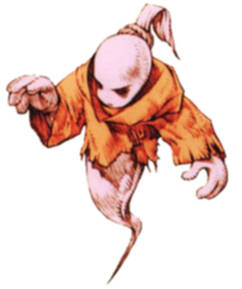
\includegraphics[width=0.2\textwidth]{./art/monsters/ghost.jpg}}
{
	HP: & \hfill 50 & MP: & \hfill 40\\
	STR: & \hfill 3 & DEF: & \hfill 3 \\
	MAG: & \hfill 5 & RES: & \hfill 6 \\
	AGI: & \hfill 2 & Size: & \hfill M\\
}
{
	\textbf{Touch}: 2d DMG \hfill \textbf{Weak}:\holy \hfill \textbf{Drops:} 500 Gil 
}
{
	\mtech{Zombie Touch}{4}{0r}{Single}{Weapon}{Make an Attack against the target. If you hit, he suffers Zombie for 10 rounds on top of the damage dealt.}{}	
	\mtech{Drain Touch}{5}{0r}{Single}{Weapon}{Make an Attack against the target. If you hit, increase your HP by 1d on top of the damage dealt.}{}	
}
%
%
\ofaccent{Bravery \& Faith:} 
To create more heroic moments in your adventure, you can allow characters to derive special powers from their Bravery or Faith.
Every character tracks one resource pool for each, that can hold up to 5 points.
Players roll 1d for each during character creation to determine their starting Bravery and Faith (a 6 is rounded down to a 5).
Characters recover 1 point of Bravery and 1 point of Faith whenever they go to sleep and they can never spend more than 1 point of either at once.
\textbf{Bravery} allows characters to channel their inner courage to reach beyond their usual abilities.
Characters can spend 1 point of Bravery whenever they perform a check to add 1 to the result of their roll.
They can also spend 1 point of Bravery whenever they deal any damage during combat to add 1d to the total damage dealt.
When a character's Bravery drops to 0, all of their total damage dealt is halved.
The GM can award additional points of Bravery whenever someone acts particularly heroic or deduct a point when they act cowardly.
\textbf{Faith} helps characters to overcome failures through confidence in their beliefs.
Characters can spend 1 point of Faith whenever they perform a check to re-roll one die after seeing the result.
They can also spend 1 point of Faith whenever they suffer any damage during combat to reduce the total damage suffered by 1d.
The GM can award additional points of Faith whenever someone acts in accordance to their belief system and deduct a point when they act against it.
When a character's Faith drops to 0, they have Disadvantage on every check that they perform.
%
\\\\
%
\ofaccent{Hiring Soldiers:} 
In the world of Ivalice, many capable combatants will offer their services for the right price.
As such, the party can hire paid soldiers in almost any major city to improve their combat strength.
These soldiers are controlled by the GM during battles and generally should not play a major role outside of it.
Accordingly, you also do not need to track their current experience and progression. 
For characters of greater importance, we recommend to use the standard character creation rules, if necessary you
can convert a hired soldier to a fully fledged character later on.
When using the \textbf{Bravery \& Faith} rules, a hired soldier will immediately leave the party when either their Bravery or Faith drops to 0.
On the right are some examples of soldiers that can be hired, along with their required daily salary.
As these are very common types of combatants, you can also use them as human enemies.
%
\\\\\\
%
\ofquote{"Most people have to act the roles given to them. Then again, most of them haven't even noticed they're acting."}{Delita Hyral}
%
\pagebreak\\
%
\ofmonster{Squire}{1}{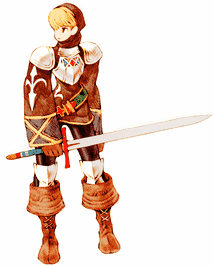
\includegraphics[width=0.22\textwidth]{./art/monsters/squire-male.png}}
{
	HP: & \hfill 15 & MP: & \hfill 8\\
	STR: & \hfill 1 & DEF: & \hfill 0 \\
	MAG: & \hfill 0 & RES: & \hfill 0 \\
	AGI: & \hfill 3 & Size: & \hfill M\\
}
{\textbf{Sword}: 1d DMG \hfill \textbf{Salary:} 25 Gil per day}
{
	\mtech{Throw Stone}{2}{0r}{Single}{3u}{The target suffers 1d damage.}{}
	\ofrow\ofaccent{Items:} 1x Potion		
}
%
\ofrow
%
\ofmonster{Chemist}{2}{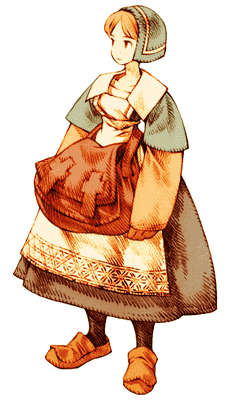
\includegraphics[width=0.14\textwidth]{./art/monsters/chemist-female.png}}
{
	HP: & \hfill 18 & MP: & \hfill 10\\
	STR: & \hfill 1 & DEF: & \hfill 1 \\
	MAG: & \hfill 0 & RES: & \hfill 1 \\
	AGI: & \hfill 2 & Size: & \hfill M\\
}
{\textbf{Knife}: 1d DMG \hfill \textbf{Salary:} 50 Gil per day}
{
	\mreaction{Auto-Potion}{Whenever an ally within 1u suffers damage, you can immediately use an Item on them.}		
	\ofrow\ofaccent{Items:} 3x Potion, 1x Phoenix Down, 1x Remedy
}
%
\ofrow
%
\ofmonster{Archer}{3}{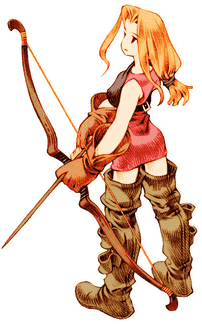
\includegraphics[width=0.16\textwidth]{./art/monsters/archer-female.png}}
{
	HP: & \hfill 27 & MP: & \hfill 14\\
	STR: & \hfill 1 & DEF: & \hfill 1 \\
	MAG: & \hfill 0 & RES: & \hfill 0 \\
	AGI: & \hfill 2 & Size: & \hfill M\\
}
{\textbf{Bow}: 2d DMG, 3u range \hfill \textbf{Salary:} 100 Gil per day}
{
	\mtech{Aim}{2}{1r}{Single}{Self}{
		On the next Attack that you perform, the target has Disadvantage on the evasion check.
	}{}	
	\ofrow\ofaccent{Items:} 2x Potion, 1x Eyedrops	
}
%
\ofrow
%
\ofmonster{Knight}{4}{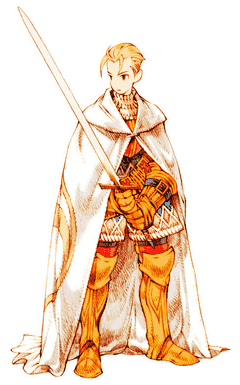
\includegraphics[width=0.17\textwidth]{./art/monsters/knight-male.png}}
{
	HP: & \hfill 38 & MP: & \hfill 20\\
	STR: & \hfill 3 & DEF: & \hfill 2 \\
	MAG: & \hfill 0 & RES: & \hfill 1 \\
	AGI: & \hfill 3 & Size: & \hfill M\\
}
{\textbf{Sword}: 2d DMG \hfill \textbf{Salary:} 150 Gil per day}
{
	\mtech{Rend Power}{5}{0r}{Single}{Weapon}{
		Make an Attack against the target.  If you hit, the damage dealt is halved and the target suffers EnSTR for 3 rounds.
	}{}	
	\mtech{Rend Magick}{5}{0r}{Single}{Weapon}{
		Make an Attack against the target.  If you hit, the damage dealt is halved and the target suffers EnMAG for 3 rounds.
	}{}	
	\ofrow\ofaccent{Items:} 1x Hi-Potion, 1x Remedy	
}